\documentclass[UTF8,14pt]{article}
\usepackage[UTF8]{ctex}
\usepackage[a4paper, margin=1in]{geometry}
\usepackage{fancyhdr}
\usepackage{enumerate}
\usepackage{subfigure}
\usepackage{amsmath}
\numberwithin{figure}{section}
\pagestyle{fancy}
\lhead{网络空间安全一班} % Top left header
\chead{可靠传输协议实验报告} % Top center head
\rhead{谢远峰3019244283} % Top right heade
\renewcommand\headrulewidth{0.2pt} % Size of the header rule
\renewcommand\footrulewidth{0.4pt} % Size of the footer rul
\usepackage{amsmath}
\usepackage{subfigure}
\usepackage{titlesec}
\usepackage{fancyhdr} % Required for custom headers
\usepackage{lastpage} % Required to determine the last page for the footer
\usepackage{subfig,graphicx} % Required to insert images
\usepackage{enumitem}


% \cfoot{第\ \thepage\ 页}
% \titleformat{\section}{\huge\bfseries}{1em}{}
\titleformat{\section}[hang]{\Large \bfseries}{\vspace{-1cm}\arabic{section}}{0.8em}{}[]
\titleformat{\subsection}[hang]{\large \bfseries}{\arabic{subsection} }{0.4em}{}[]
\titleformat{\subsubsection}[block]{\large \bfseries}{ \arabic{subsubsection} }{0.1em}{}[]

% \setlength{\parskip}{2mm}
\setenumerate[1]{itemsep=0pt,partopsep=0pt,parsep=\parskip,topsep=0pt}
\setitemize[1]{itemsep=0pt,partopsep=0pt,parsep=\parskip,topsep=0pt}
\setdescription{itemsep=0pt,partopsep=0pt,parsep=\parskip,topsep=0pt}
\Huge
\title{可靠传输协议实验报告}
\begin{document}

\begin{titlepage}
      \begin{center}
            \begin{figure}[ht]
                  \centering
                  
\includegraphics[width=10cm,height=9.5cm]{figures/封面.png}
            \end{figure}
            \line(1,0){300}\\
            [0.65cm]
            \Huge{\bfseries 可靠传输协议实验报告 }\\
            \line(1,0){300}\\
            \huge {停等协议及回退N协议\\
                  \today}\\
            [3.5cm]
            \LARGE{
                  \begin{tabular}{rl}
                        学院 :        & 智能与计算学部 \\
                        班级 :        & 网络安全一班   \\
                        姓名        : & 谢远峰         \\
                        学号       :  & 3019244283
                  \end{tabular}
            }
      \end{center}

\end{titlepage}
\clearpage

\section{比特交替协议}
\subsection{原理}
\vspace*{-0.5cm}
\begin{center}
      \begin{figure}[ht]
            \centering
            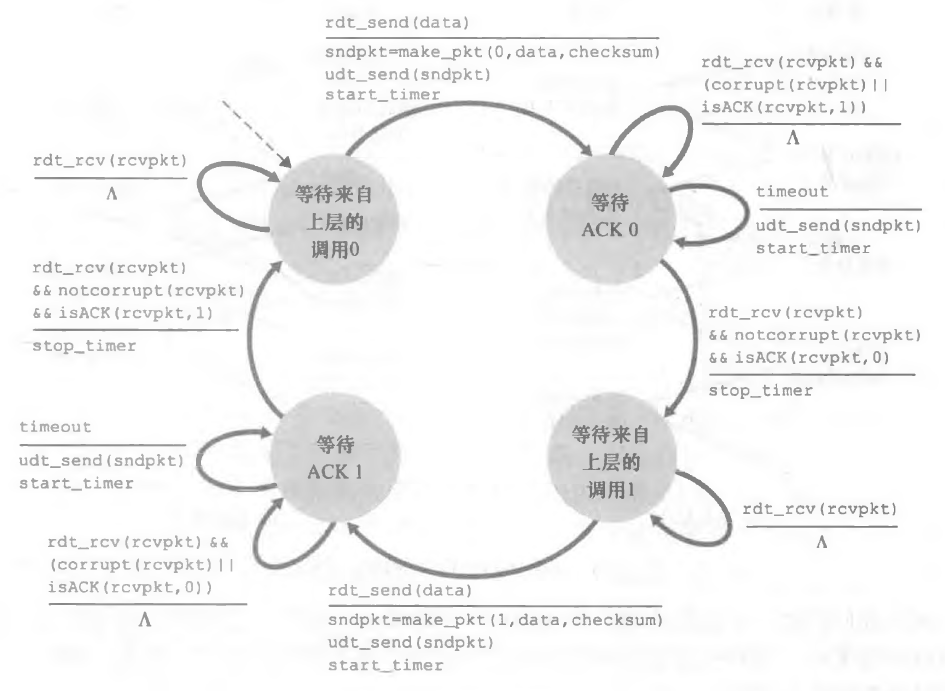
\includegraphics[width=12.6cm,height=9cm]{figures/abp.png}
      \end{figure}
\end{center}
\vspace*{-1cm}

停止等待协议是tcp保证传输可靠的重要途径,“停止等待”就是指发送完一个分组就停止发送,等待对方的确认,只有对方确认过,才发送下一个分组。在停止-等待协议中,源站发送单个帧后必须等待确认,在目的站的回答到达源站之前,源站不能发送其他的数据帧。从滑动窗口机制的角度来看,停止-等待协议相当于发送窗口和接收窗口大小均为1的滑动窗口协议。
\subsection{过程}
\vspace{-0.5cm}
\begin{figure}[!htbp]
      \centering
      \begin{minipage}[!ht]{0.49\textwidth}
            \centering
            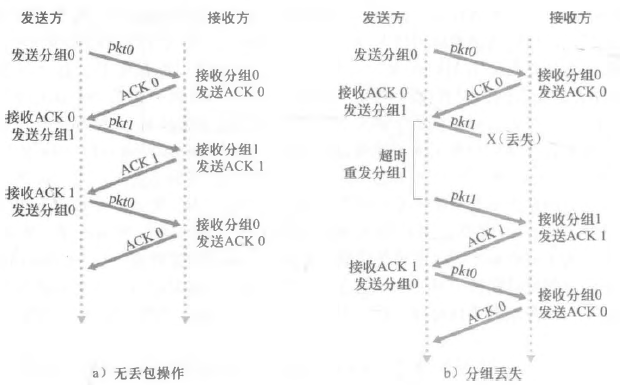
\includegraphics[width=7cm,height=5.5cm]{figures/abp1_2.png}
            % \caption{World Map}
      \end{minipage}
      \begin{minipage}[!ht]{0.49\textwidth}
            \centering
            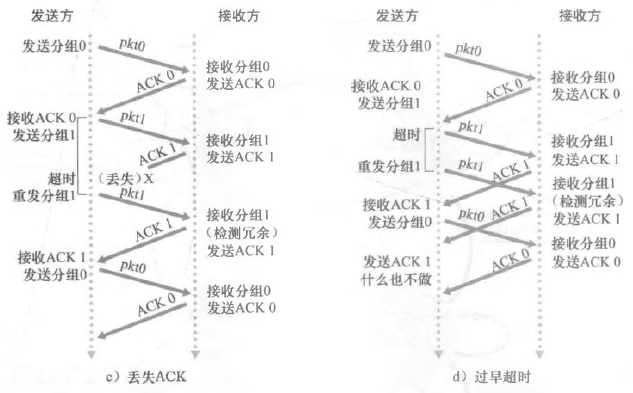
\includegraphics[width=7cm,height=5.5cm]{figures/abp1_3.png}
            % \caption{Concrete and Constructions}
      \end{minipage}
      \caption{情况列举}
\end{figure}

\begin{enumerate}
      \setlength{\parskip}{-5mm}
      \item {无差错情况}\\
            发送方发送分组,接收方在规定时间内收到,并且回复确认.发送方再次发送\\
      \item {分组丢失}\\
            发送方发送分组,接收方没有收到分组,那么接收方不会发出确认,只要发送方过一段时间没有收到确认,就认为刚才的分组丢了,那么发送方就会再次发送.\\
      \item {确认丢失}\\
            发送方发送成功,接收方接收成功,确认分组也被发送,但是分组丢失,那么到了等待时间,发送方没有收到确认,又会发送分组过去,此时接收方前面已经收到了分组,那么此时接收方要做的事就是:丢弃分组,重新发送确认.\\
      \item {传送丢失}\\
            发送方发送成功,接收方接收成功,确认分组也被发送,没有丢失,但是由于传输太慢,等到了发送方设置的时间,发送方又会重新发送分组,此时接收方要做的事情:丢弃分组,重新发送确认. 发送方如果收到两个或者多个确认,就停止发送,丢弃其他确认.
\end{enumerate}
\vspace*{-0.5cm}
\subsection{算法实现规划}
\begin{itemize}
      \setlength{\parskip}{-5mm}
      \item {明确发送包的发送顺序:\quad}A发送端接收应用层消息,进行打包转到传输层,B接受端接收发送的包并进行校验,如果匹配则进行拆解等到消息上传至应用层,否则进行消息回传,通知A发送方进行包的重传\\
      \item {A发送端进行初始化:\quad}确立发送方状态(等待应用层消息/等待接受端的反馈),发送包的序列号(0/1),计时器,打包的备份\\
      \item {B接收端进行初始化:\quad}确定待接收的序列号\\
      \item {检验和的计算:\quad}无论是发送方还是接收方,都需要对包进行校验和的计算:发送方计算序列号、消息的校验和(ACK为默认为0);接收方需要对消息进行校验\\
      \item {NAK/ACK的发送:\quad}若通过校验,赋值ACK,否则,赋值最近一次成功的ACK,重新计算校验和并发送\\
      \item {超时处理:\quad}计时超限,发送备份包,并重新计时\\
      \item {异常处理:\quad}发送方接收应用层消息前,需判断当前状态是否为等待消息;发送方接收ACK时需判断是否处于等待ACK状态;接收序列号不匹配时,需进行重传处理\\
      \item {双向传输:\quad}在包中添加发送方状态信息,并在初始化阶段,分别建立接收端和发送端,在收发函数中,根据包内含有的发送方的信息进行判定。
\end{itemize}
\vspace*{-0.5cm}
\subsection{实现具体细节}
单向传输
\begin{itemize}
      \setlength{\parskip}{-5mm}
      \item {初始化:\quad}A发送端默认初始状态为等待消息输入,发送的序列号为0,计时为20;B接收端默认待接收的序列号为0\\
      \item {A发送方发送:\quad}判定发送方状态,初始化消息报,装载序列号,拷贝消息进入包中,默认ACK为0,计算校验和,标记发送方,备份消息包,设置期待接收的ACK,发送包至传输端,开始计时。\\
      \item {B接收方接收:\quad}判定包传输途中消息是否出错,判定包序列号是否正确,若未通过发送NAK,否则发送ACK,更新待接收的序列号\\
      \item {A发送方接收ACK:\quad}判定发送方状态,校验和判定,序列号正确性判定,停止计时,更新待发送的序列号,更新发送方的状态\\
\end{itemize}
\vspace{-1cm}

\subsection{问题复现}
\begin{itemize}
      \setlength{\parskip}{-5mm}
      \item {函数格式的更改:\quad}由于底层函数的声明不同于大众化写法,故在文件开始进行正确声明\\
      \item {消息发送语句的次序问题:\quad}先赋值后计算校验和,而后发送,计时,最后转换状态,顺序错乱可能导致消息错误率过高,超时频率增强\\
      \item {双向传输的书写:\quad}在发送包中添加信息,需要在底层同样增加信息的声明初始化,同时A,B都应同时设置收发两种状态,并在函数中进行发送方的确认\\
      \item {函数传参的正确书写:\quad}双向传输中,0,1参数的错误需借助函数内部自定义的输出锁定错误位置\\
\end{itemize}
\vspace*{-0.8cm}
\newpage
\subsection{仿真结果}
\vspace*{-1cm}
\begin{figure}[!htbp]
      \centering
      \setlength{\abovecaptionskip}{0.cm}
      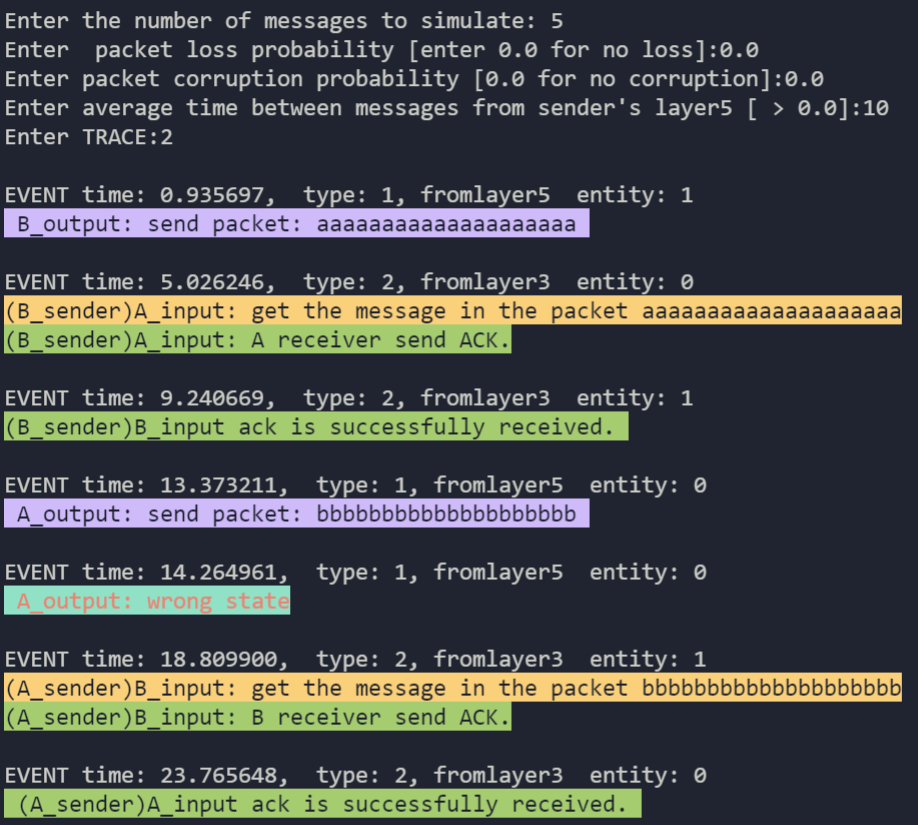
\includegraphics[width=8.9cm,height=8cm]{figures/result2.png}
      \caption{实现理想状态下的消息传输}
\end{figure}

以单向传输为例,A为发送方,B为接收方,设定发送消息为3,丢包率和错包率为0,消息的发送间隔为1000个时间单位,进行过程消息追踪,消息能够成功进行传输
\vspace*{-0.5cm}
\subsection{算法功能/性能测试:双向传输展示}
\vspace*{-0.5cm}
\begin{figure}[!htb]
      \centering
      \setlength{\abovecaptionskip}{0.cm}
      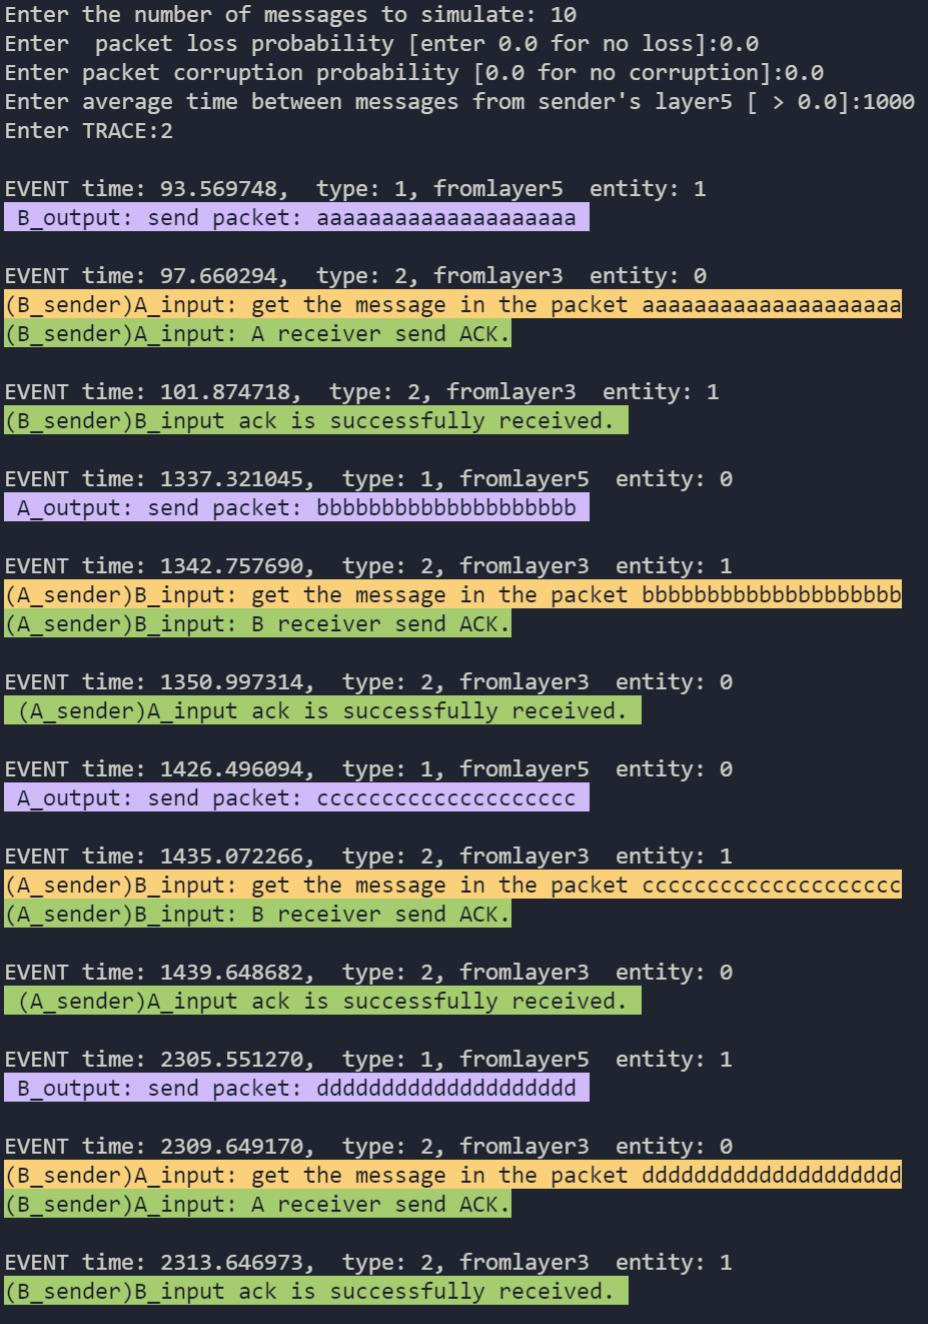
\includegraphics[width=7.70cm,height=11cm]{figures/result1.png}
      \caption{无loss,error}
\end{figure}

双向传输,A作为发送方发送b,c两个串,B作为发送方发送a,d两个串,正常运行
\clearpage
\begin{center}
      \begin{figure}[!ht]
            \centering
            % \setlength{\abovecaptionskip}{0.cm}
            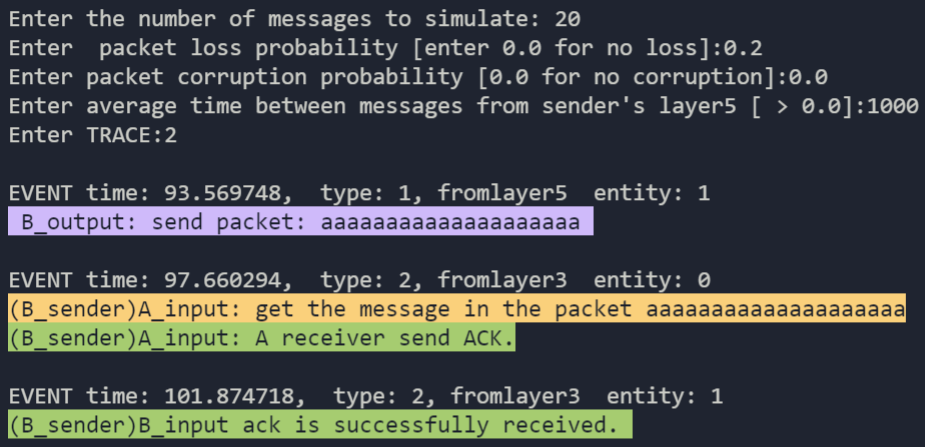
\includegraphics[width=15cm,height=7.24cm]{figures/result3_1.png}
            \caption{数据包、ACK/NAK包有loss}
      \end{figure}
      \begin{figure}[!ht]
            \centering
            % \setlength{\abovecaptionskip}{0.cm}
            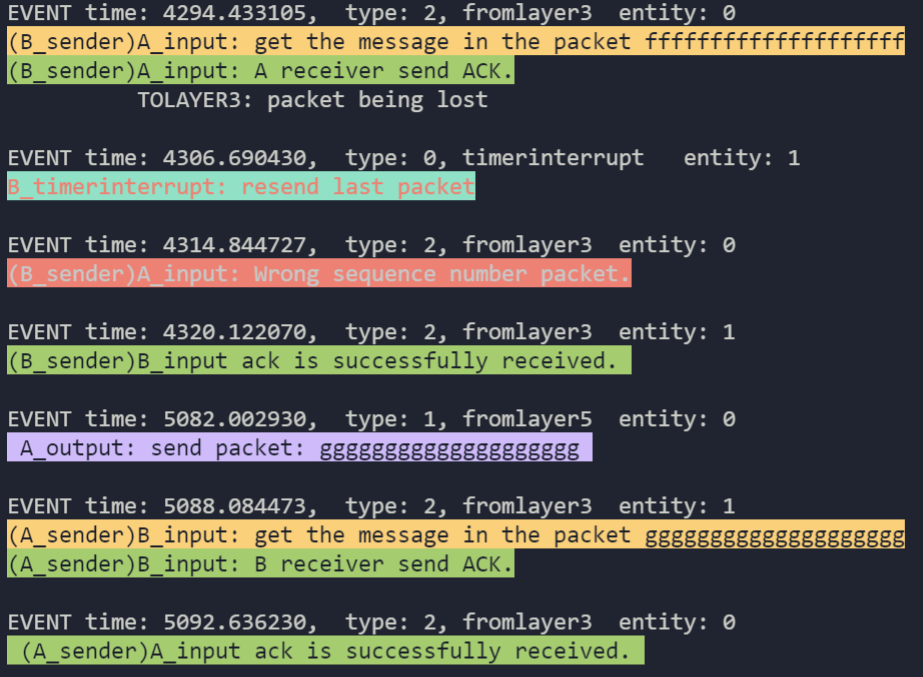
\includegraphics[width=15cm,height=11cm]{figures/result3_2.png}
            \caption{数据包、ACK/NAK包有loss}
      \end{figure}
\end{center}
\vspace{-1.5cm}

数据包、ACK/NAK包有丢失状态,测试采用20个样例,包的丢失率为20\%,无包的错误率,应用层消息的发送间隔为1000个时间单位,进行信息的追踪。B发送F串时,返回的ACK丢失,造成B的计时器超时重传,A接收方预期收到的序列号不匹配,发送最新匹配成功的ACK包,B发送方成功进行接收。A发送g串,B成功接收并返回ACK,A成功接收。
\newpage
\begin{figure}[!htbp]
      \centering
      % \setlength{\abovecaptionskip}{0.cm}
      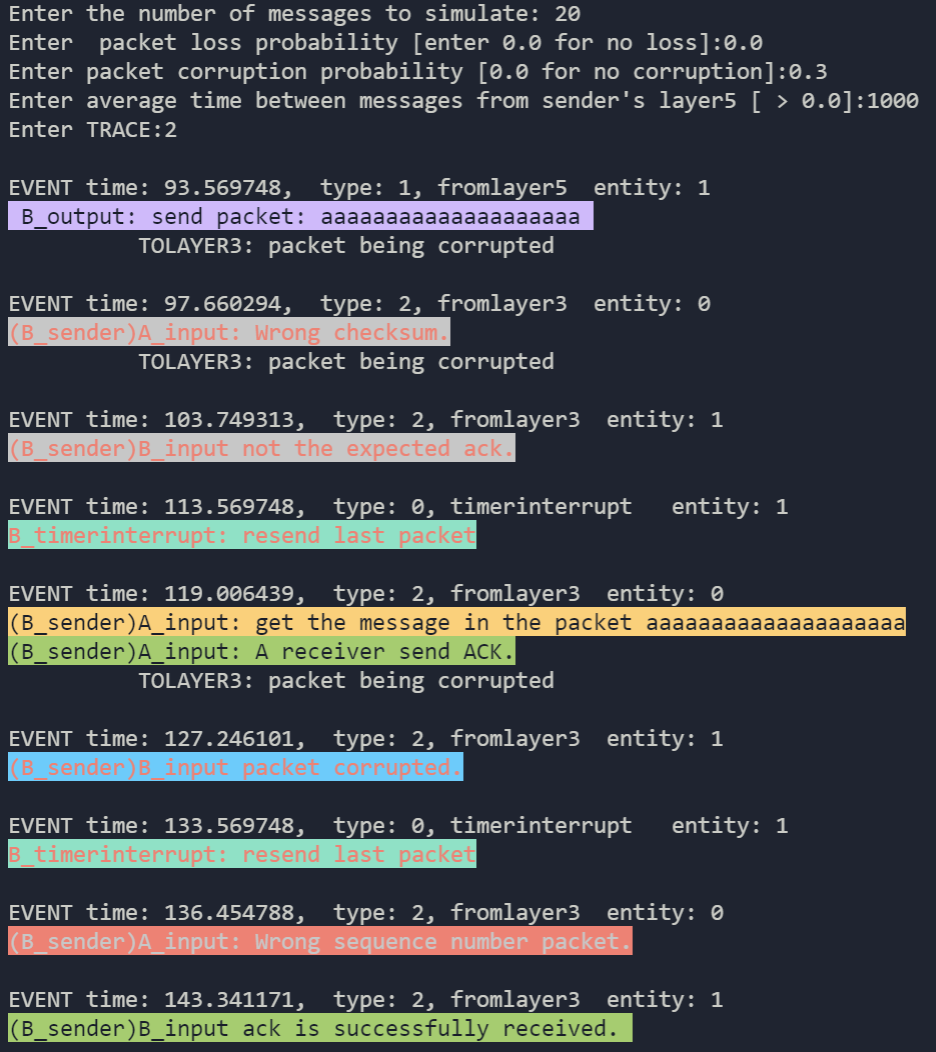
\includegraphics[width=15cm,height=16.85cm]{figures/result4_1.png}
      \caption{数据包、ACK/NAK包有error}
      % \includegraphics[width=14.5cm,height=23cm]{result4_2.png}
      % \caption{数据包、ACK/NAK包有error}
\end{figure}

数据包、ACK/NAK包有错误状态,测试采用20个样例,仅截取部分进行说明,包的错误率为30\%,无包的丢失率,应用层消息的发送间隔为1000个时间单位,进行信息的追踪。B发送a串时,包发送比特错误,A接收方预期收到的序列号不匹配,B计时器超时重新发送,A接收方成功接收并返回ACK。
% \vspace*{-1cm}
\clearpage
\section{回退N协议}
\subsection{原理}
\vspace{-0.5cm}
\begin{figure}[!htbp]
      \centering
      \begin{minipage}[!ht]{0.59\textwidth}
            \centering
            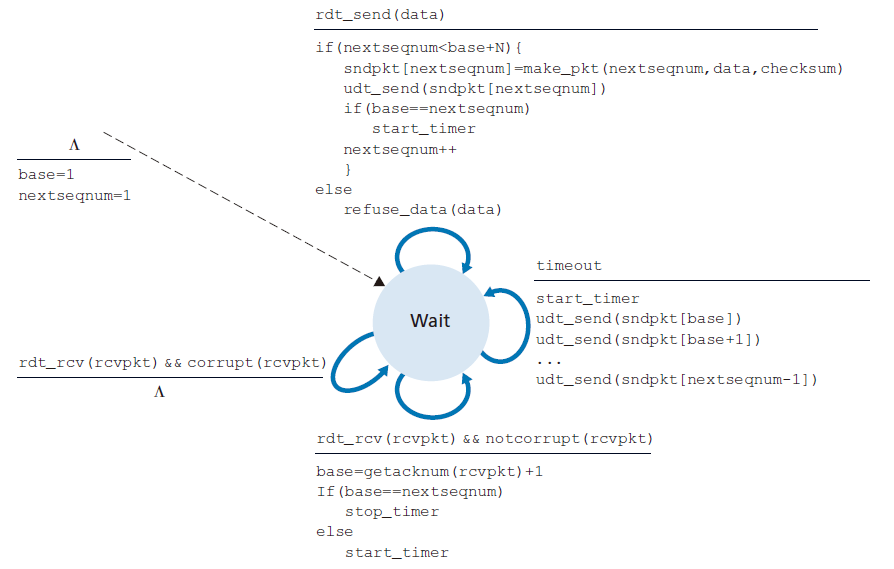
\includegraphics[width=8cm,height=5.5cm]{figures/gbn1.png}
            % \caption{World Map}
      \end{minipage}
      \begin{minipage}[!ht]{0.39\textwidth}
            \centering
            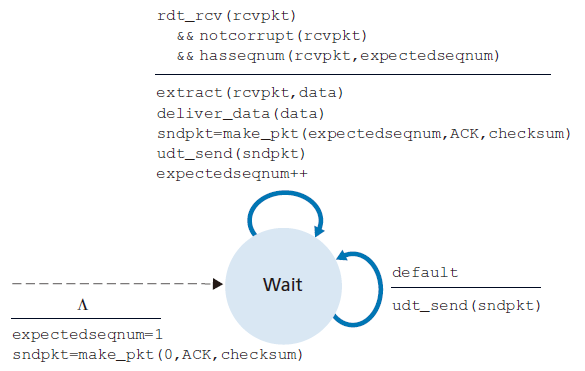
\includegraphics[width=6cm,height=4.3cm]{figures/gbn2.png}
            % \caption{Concrete and Constructions}
      \end{minipage}
      \caption{情况列举}
\end{figure}

GBN是属于传输层的协议,它负责接收应用层传来的数据,将应用层的数据报发送到目标IP和端口

滑动窗口: 假设在序号空间内,划分一个长度为N的子区间,这个区间内包含了已经被发送但未收到确认的分组的序号以及可以被立即发送的分组的序号,这个区间的长度就被称为窗口长度。(随着发送方对ACK的接收,窗口不断的向前移动,并且窗口的大小是可变的)

接收方只需要按序接收分组,对于比当前分组序号还要大的分组则直接丢弃。假设接收方正在等待接收分组n,而分组n+1却已经到达了,于是,分组n+1被直接丢弃,所以发送方并不会出现在连续发送分组n,分组n+1之后,而分组n+1的ACK却比分组n的ACK更早到达发送方的情况。
\subsection{过程}
\begin{figure}[!htbp]
      \centering
      \setlength{\abovecaptionskip}{0.cm}
      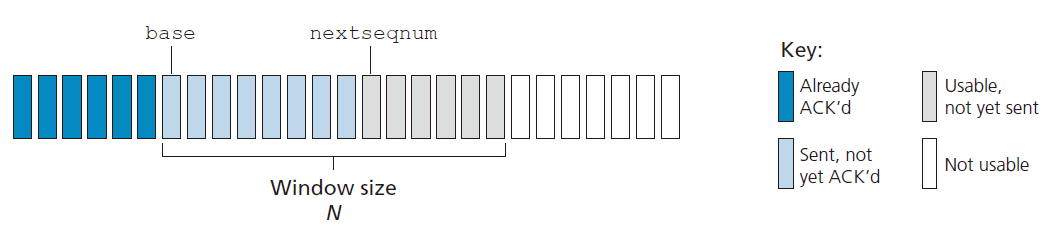
\includegraphics[width=10.55cm,height=2.27cm]{figures/gbn3.png}
      \caption{消息包的分类}
\end{figure}

GBN协议的事件判断:
\begin{enumerate}
      \setlength{\parskip}{-5mm}
      \item $[0,send\_{}base-1]:$已发送并且收到确认了的序列号\\
      \item $[send\_{}base,nextseqnum - 1]:$已发送但未收到确认了的序列号\\
      \item $[nextseqnum, send\_{}base + N - 1]:$可被用于发送新分组的序列号\\
      \item 大于等于$[send\_{}base + N]:$不能使用的序列号\\
\end{enumerate}

协议中,已发送但未被确认的分组数目不能超过N。因此N可以看做是从第一个已发送但未被确认的序号(就是基序号)开始的长为N的序号窗口,也称为发送窗口。随着分组被确认,该窗口逐渐滑动,$send\_ base$增加,但是其大小不变,因此该协议也称为滑动窗口协议。假设序号空间总大小为X,所有的序号计算都要对X取模。

对于超时的触发,GBN协议会将当前所有已发送但未被确认的分组重传,即如果当前窗口内都是已发送但未被确认的分组,一旦定时器发现窗口内的第一个分组超时,则窗口内所有分组都要被重传。每次当发送方收到一个ACK的时候,定时器都会被重置。

\subsection{算法实现规划}
发送方需要处理事件
\begin{enumerate}
      \setlength{\parskip}{-5mm}
      \item 上层调用进行发送:当发送数据时,首先判断发送窗口是否已满,只有不满时才会启动发送,如果满了则不能发送或者缓存或者通知调用者,这取决于实现。(判满)\\
      \item 收到ACK:如果收到了分组n的ACK,并且分组n的序号在$[send\_{}base,  nextseqnum - 1]$之间,则更新send$\_$base。GBN协议采用累积确认,含义是如果发送方接收到了对分组n的确认,则表明分组n之前的所有分组都已经被接收。\\
      \item 超时事件:GBN协议名字来自该协议对分组丢失或超时事件的处理。如果分组丢失或者指定的时间内仍未收到对已发送但是未收到确认的分组的确认,则发送方重传$[send\_{}base, nextseqnum-1]$之间的所有分组。实现中可以只为序号为send$\_{}$base的分组启动一个定时器,如果send$\_{}$base被更新就重启send$\_{}$base相关的定时器,如果没有已经被发送但未被确认的分组,则关闭定时器。
\end{enumerate}
\vspace{0.8cm}

接收方需要处理事件

接收方接收到分组n时,如果n是按序接收的,即分组n之前的所有分组都已经到达,则发送一个对分组n的确认,并将分组提交给上层。所有其它情况,接收方都丢弃分组,并重传对最后一个按序接收的分组的确认。这种设计简化了接收方接收缓存的设计,同时被丢弃的分组早晚都会被重传,因而可靠性也是有保证的。
GBN协议的接收方只维护了一个期望收到的下一个序号的信息,并保存在expectedseqnum中,在expectedseqnum之前的所有分组都已经被正确接收并提交给了上层。接收方具体的行为如下:
\begin{enumerate}
      \setlength{\parskip}{-5mm}
      \item 如果收到的分组的序号与expectedseqnum相同,则将分组提交给上层,并更新它的值为下一个期望收到的序号。\\
      \item 如果收到的分组的序号大于expectedseqnum,就丢弃分组。\\
      \item 如果收到的分组的序号小于expectedseqnum,就重传对最后一个按序接收的分组的确认。由于GBN是累积确认的,因此该确认可以确保发送窗口可以向前移动。送但未被确认的分组,则关闭定时器。
\end{enumerate}
\subsection{实现具体细节}
\begin{itemize}
      \setlength{\parskip}{-5mm}
      \item {发送方信息确定:\quad}先赋值后计算校验和,而后发送,计时,最后转换状态,顺序错乱可能导致消息错误率过高,超时频率增强\\
      \item {接收方信息确定:\quad}在发送包中添加信息,需要在底层同样增加信息的声明初始化,同时A,B都应同时设置收发两种状态,并在函数中进行发送方的确认\\
      \item {宏定义:\quad}定义窗口大小,序列号带线啊哦\\
      \item {发送方窗口发送:\quad}进行缓冲区长度判定,初始化发送包,获取序列号,装载应用层消息,定义发送端信息,初始化ACK值,计算校验和,更新发送端缓冲区末端,发送窗口内部消息\\
      \item {接收方窗口接收:\quad}进行校验和及序列号判定,解包获取消息上传至应用层,赋值ACK,重新计算校验和,发送至网络层,更新下一次的预期序列号\\
\end{itemize}
\subsection{遭遇问题}
\begin{itemize}
      \setlength{\parskip}{-5mm}
      \item {ACK及窗口基地址的更新:\quad}将缓冲区内的标号模序列号进行运算,其中包括接收方对于ACK的赋值和发送方对于窗口基地址的更新,新的窗口基地址等于原地址与获取到ACK到基地址的距离\\
\end{itemize}
\newpage
\subsection{仿真结果}
\vspace{-0.7cm}
\begin{figure}[!htbp]
      \centering
      \setlength{\abovecaptionskip}{0.cm}
      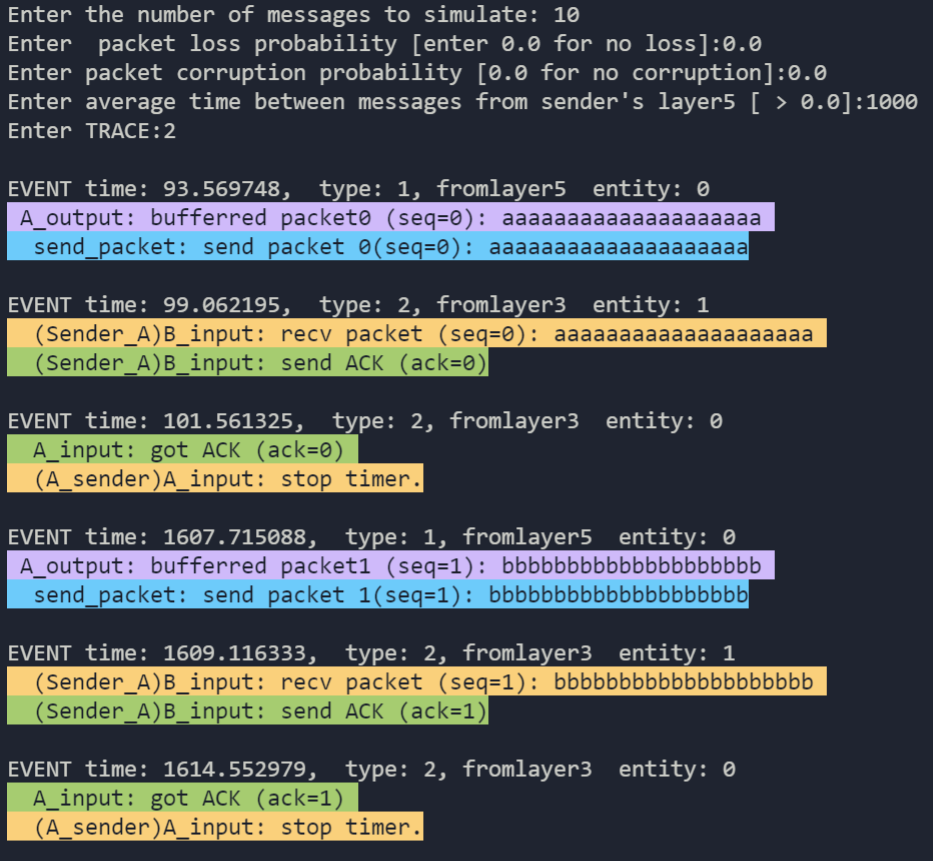
\includegraphics[width=12cm,height=11.07cm]{figures/gbn.png}
      \caption{消息包的分类}
\end{figure}
以单向传输为例,A为发送方,B为接收方,设定发送消息为3,丢包率和错包率为0,消息的发送间隔为1000个时间单位,进行过程消息追踪,消息能够成功进行传输
\vspace{-0.5cm}
\subsection{算法功能/性能测试}
\vspace{-0.5cm}
\begin{figure}[!htbp]
      \centering
      \setlength{\abovecaptionskip}{0.cm}
      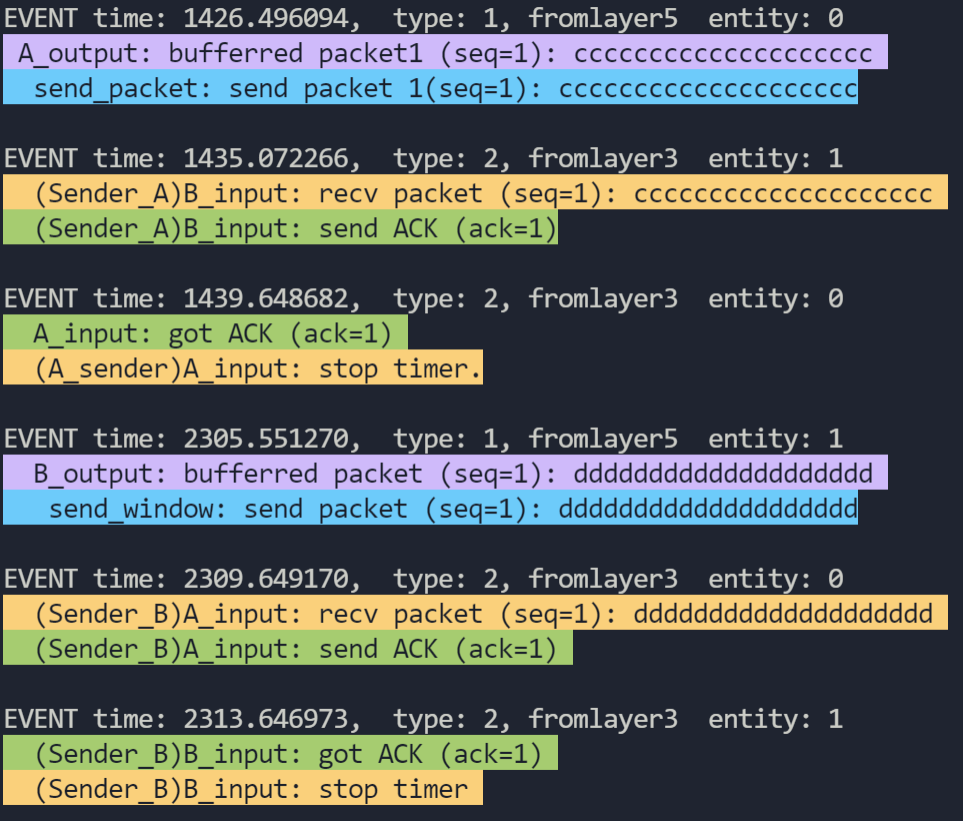
\includegraphics[width=12cm,height=9.54cm]{figures/gbn0_1.png}
      \caption{无loss,error}
\end{figure}

\newpage
\begin{figure}[!htbp]
      \centering
      \setlength{\abovecaptionskip}{0.cm}
      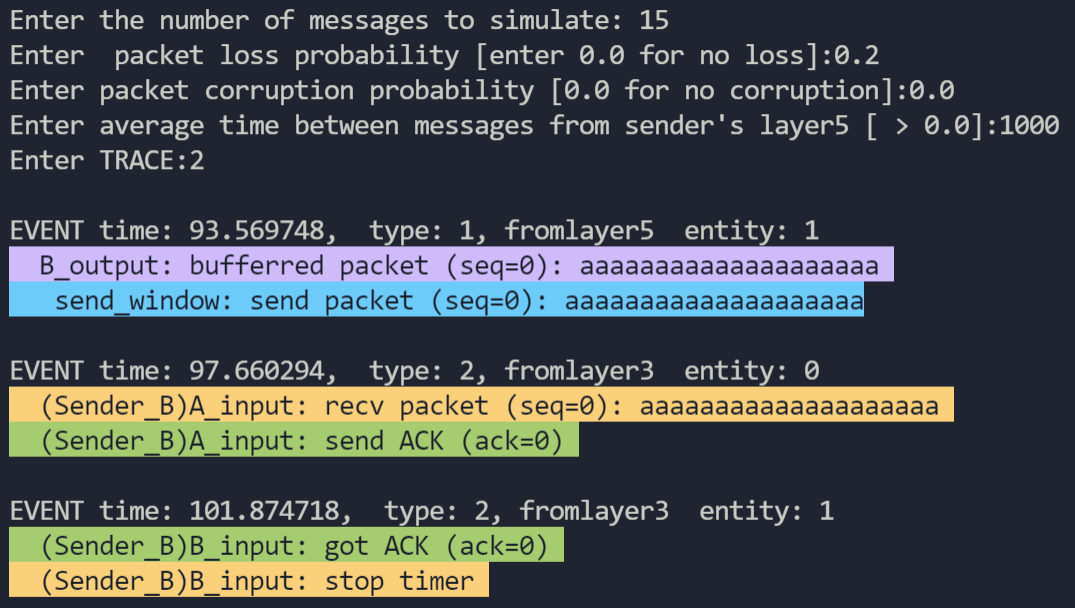
\includegraphics[width=15cm,height=8.48cm]{figures/gbn1_1.png}
      % \setlength{\abovecaptionskip}{0.cm}
      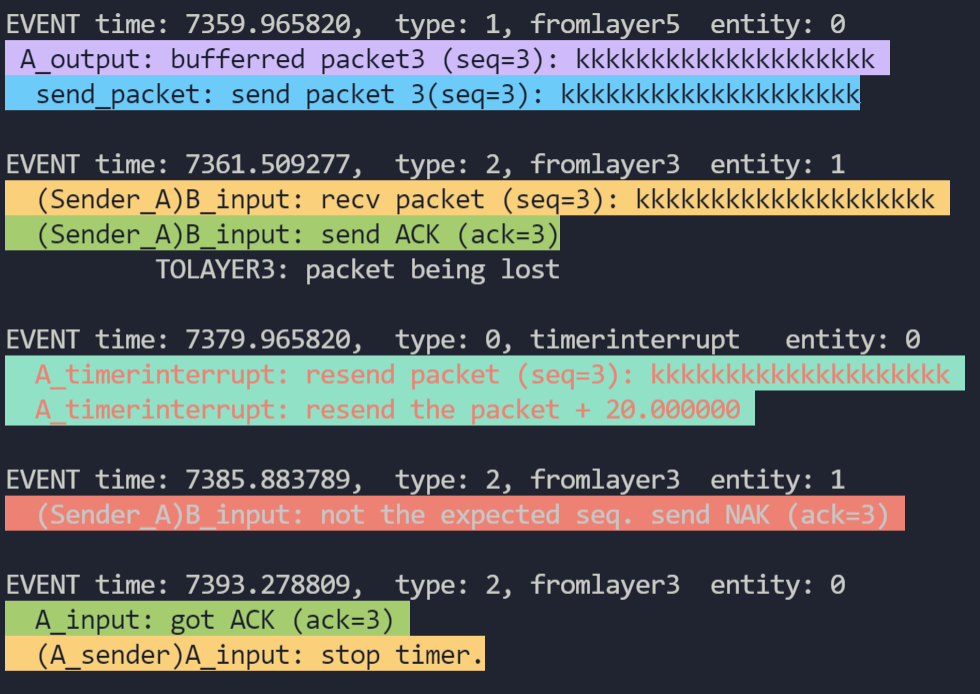
\includegraphics[width=15cm,height=10.62cm]{figures/gbn1_2.png}
      \caption{有loss,无error 测试1}
\end{figure}

双向传输,b作为发送方发送a串,首次传输的包发生丢失,B收到NAK信息,B重传,A成功接收,返回ACK丢失,B重传,A返回NAK,B收到对应的ACK信息。
\newpage
\begin{figure}[!htbp]
      \centering
      \setlength{\abovecaptionskip}{0.cm}
      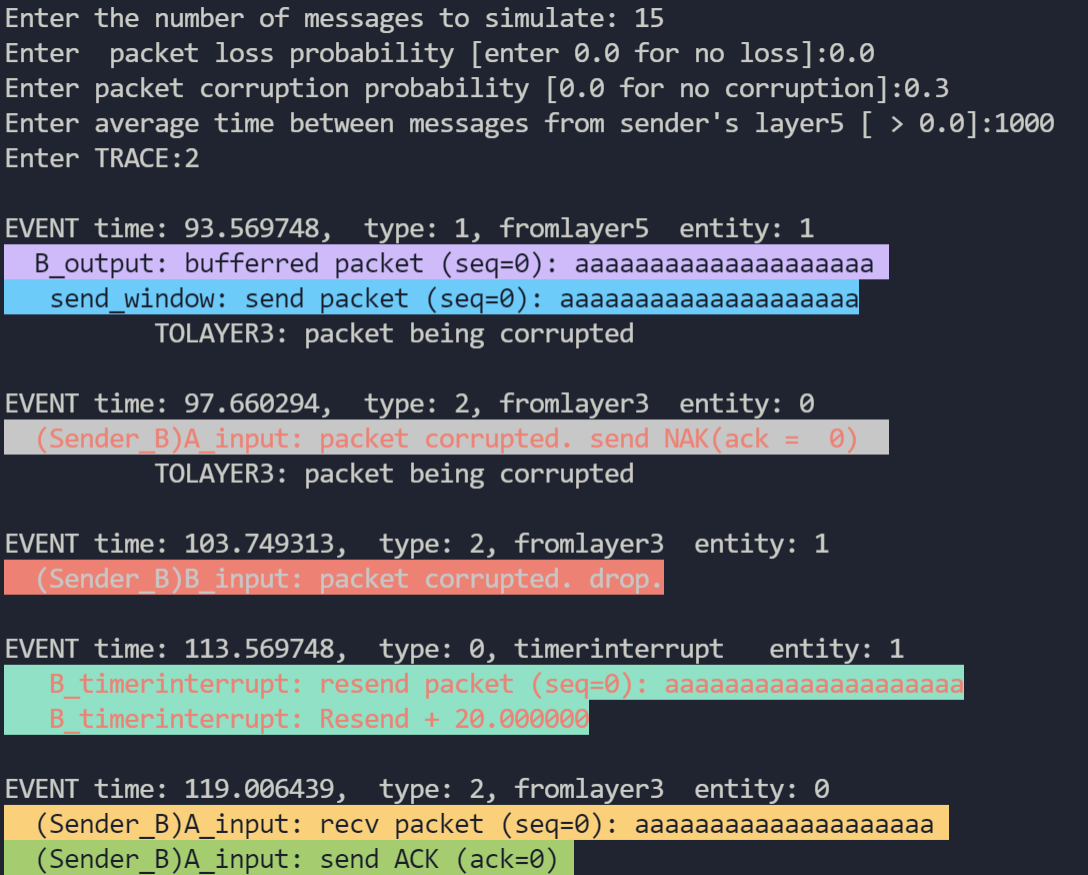
\includegraphics[width=15cm,height=12.06cm]{figures/gbn2_1.png}
      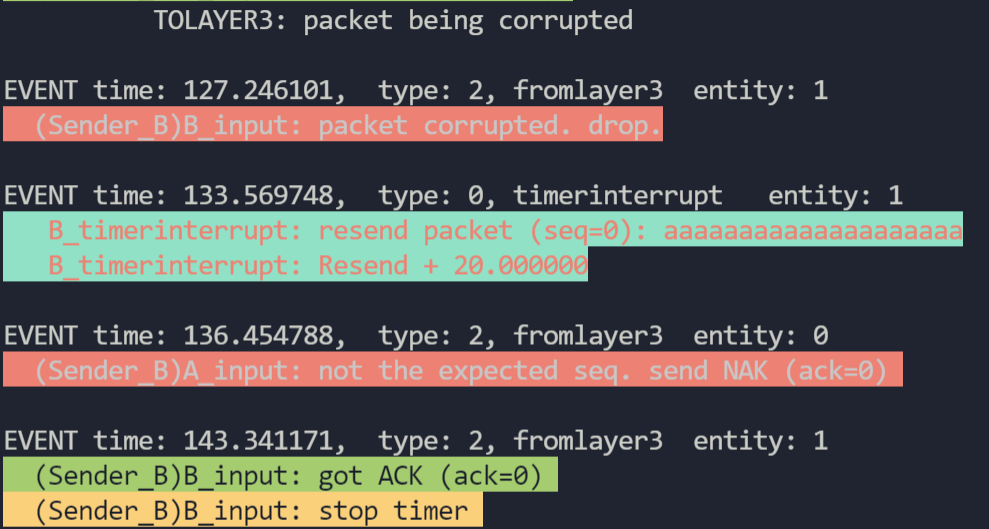
\includegraphics[width=15cm,height=8.89cm]{figures/gbn2_2.png}
      \caption{无loss,有error}
\end{figure}

双向传输,b作为发送方发送a串,首次传输的包发生错误,B收到NAK信息,B重传,A成功接收,返回ACK错误,B重传,A返回NAK,B收到对应的ACK信息。
\newpage
\section{分析和总结}
对于比特交换协议,由于其停等的特性,导致数据包在传输过程中发生丢失或错误时,消息的收发效率会大大降低。

对于回退N协议,因其具有流水线的机制,采用滑动窗口的方法确保在短时间内同时发送多个数据包,在一定程度上提高了传输效率。

对于输出消息的颜色设置能够将传输过程更加清晰地呈现。由单向传输转换为双向传输时,需要对底层传输代码进行适当的发送发信息添加。
\end{document}